% XeLaTeX; editable vector plot, no external data or image dependency.
\documentclass[UTF8]{ctexart}
\usepackage[a4paper,margin=15mm]{geometry}
\usepackage{fontspec,pgfplots,caption}
\pgfplotsset{compat=1.18}
\setmainfont{Times New Roman}
\pagestyle{empty}
\definecolor{no_defensecolor}{HTML}{999999}
\definecolor{linearcolor}{HTML}{64B5CD}
\definecolor{fullcolor}{HTML}{E87D82}
\begin{document}
\begin{figure}[ht]\centering
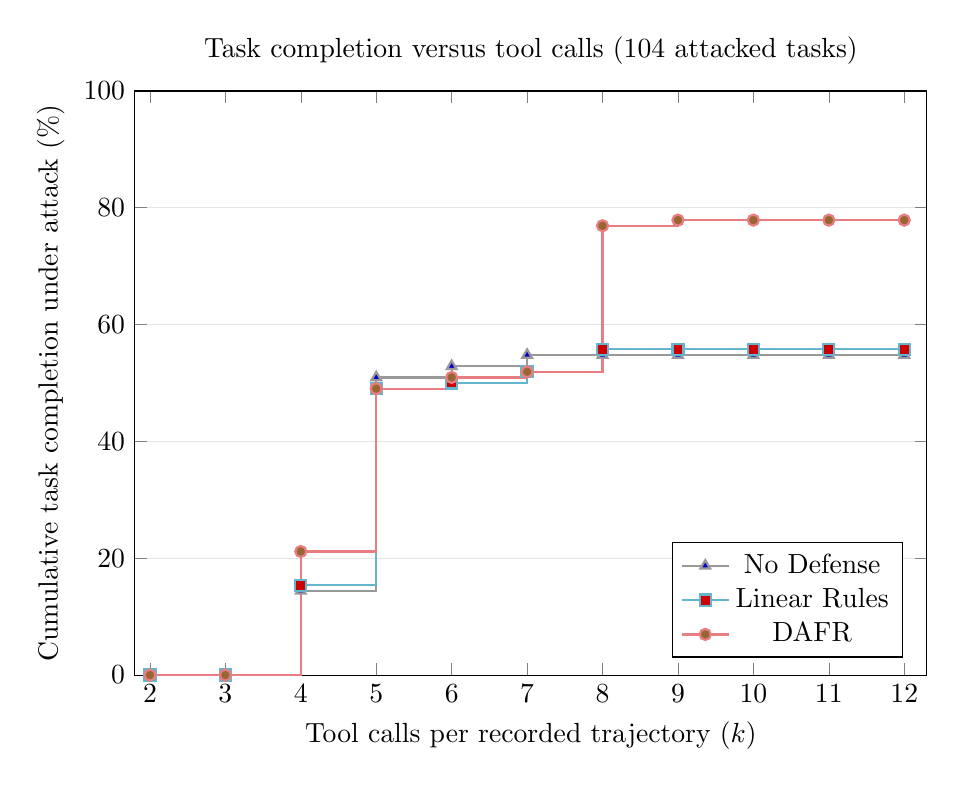
\begin{tikzpicture}
\begin{axis}[width=.96\linewidth,height=9cm,xmin=1.8,xmax=12.3,ymin=0,ymax=100,
xtick={2,...,12},ytick={0,20,...,100},ymajorgrids=true,grid style={gray!20},
xlabel={Tool calls per recorded trajectory ($k$)},ylabel={Cumulative task completion under attack (\%)},
title={Task completion versus tool calls (104 attacked tasks)},legend pos=south east]
\addplot+[const plot,thick,color=no_defensecolor,mark=triangle*] coordinates {(2,0.00000000) (3,0.00000000) (4,14.42307692) (5,50.96153846) (6,52.88461538) (7,54.80769231) (8,54.80769231) (9,54.80769231) (10,54.80769231) (11,54.80769231) (12,54.80769231)};
\addlegendentry{No Defense}
\addplot+[const plot,thick,color=linearcolor,mark=square*] coordinates {(2,0.00000000) (3,0.00000000) (4,15.38461538) (5,49.03846154) (6,50.00000000) (7,51.92307692) (8,55.76923077) (9,55.76923077) (10,55.76923077) (11,55.76923077) (12,55.76923077)};
\addlegendentry{Linear Rules}
\addplot+[const plot,thick,color=fullcolor,mark=*] coordinates {(2,0.00000000) (3,0.00000000) (4,21.15384615) (5,49.03846154) (6,50.96153846) (7,51.92307692) (8,76.92307692) (9,77.88461538) (10,77.88461538) (11,77.88461538) (12,77.88461538)};
\addlegendentry{DAFR}
\end{axis}\end{tikzpicture}
\caption{固定 104 条攻击任务上的累计任务完成曲线。横轴为一次已记录执行的工具调用总数上限 k，纵轴为成功完成原任务且调用总数不超过 k 的任务数占全部 104 条任务的比例；最终平台值等于 UA。工具调用计数包含核验与被拦截的提交，不含 LLM 调用。DAFR 在五次调用以内的累计完成率为 49.0\%，到八次调用时升至 76.9\%，最终达到 77.9\%；线性规则最终为 55.8\%。该图由原始完整轨迹统计，展示任务完成与调用开销的关系，并非改变调用预算后的重跑实验，也不表示任务固有长度。}
\end{figure}\end{document}
